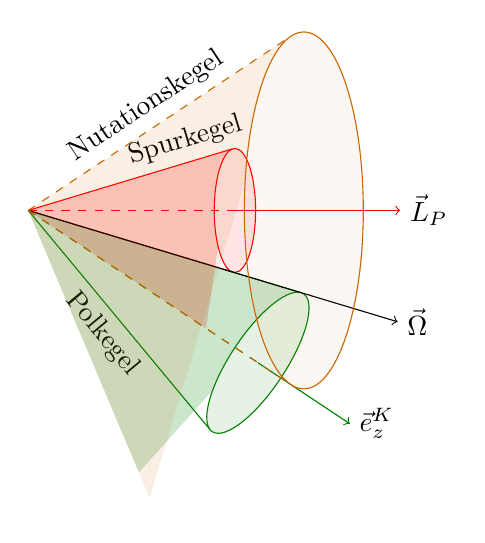
\begin{tikzpicture}[scale=.35]
	% Spurkegel
	\begin{scope}[scale=.75,draw=red]
		\filldraw[fill opacity=.1,color=red] (10,0) ellipse (1 and 3);
		\draw[rotate=-16.775] (0,0) -- (10.32,0);
		\draw[rotate=16.775] (0,0) -- (10.32,0) node[rotate=16.775,pos=.8,above] {Spurkegel};
		\draw[dashed] (0,0) -- (10,0);
		\draw[->] (10,0) -- (18,0) node[right] {$\vec{L}_P$};
		\begin{scope}[even odd rule,fill opacity=.2,color=red]
			\clip (10,0) ellipse (1 and 3) (0,0) to[rotate=16.775] (11,0) to[rotate=-33.55] (11,0) -- cycle; 
			\fill (0,0) to[rotate=16.775] (10.32,0) to[rotate=-33.55] (10.32,0) -- cycle;
		\end{scope}
	\end{scope}
	% Polkegel
	\begin{scope}[rotate=-33.55,draw=green!50!black]
		\filldraw[fill opacity=.1,color=green!50!black] (10,0) ellipse (1 and 3);
		\draw[rotate=-16.775,color=black,draw=green!50!black] (0,0) -- (10.32,0) node[rotate=-50.325,pos=.5,below] {Polkegel};
		\draw[rotate=16.775] (7.5,0) -- (10.32,0);
		\draw[dashed] (0,0) -- (10,0);
		\filldraw[->] (10,0) -- (14,0);
		\draw[fill opacity=1,color=black] (14,0) node[right] {$\vec{e}_z^K$};
		\begin{scope}[even odd rule,fill opacity=.2,color=green!50!black]
			\clip (10,0) ellipse (1 and 3) (0,0) to[rotate=16.775] (11,0) to[rotate=-33.55] (11,0) -- cycle;
			\fill (0,0) to[rotate=16.775] (10.32,0) to[rotate=-33.55] (10.32,0) -- cycle;
		\end{scope}
	\end{scope}
	% Omega
	\begin{scope}[rotate=-16.775]
		\draw[->] (0,0) -- (14,0) node[right] {$\vec\Omega$};
	\end{scope}
	% Nutkegel
	\begin{scope}[draw=orange!80!black]
		\draw[dashed,rotate=33.55] (0,0) -- (11.32,0) node[pos=.5,above,rotate=33.55] {Nutationskegel};
		\draw[dashed,rotate=-33.55] (0,0) -- (11.32,0);
		\filldraw[fill=orange!80!black,fill opacity=.05] (10,0) ellipse (2.158 and 6.475);
		\begin{scope}[even odd rule,fill opacity=.1,color=orange!80!black]
			\clip (10,0) ellipse (2.158 and 6.475) (0,0) to[rotate=33.55] (12,0) to[rotate=-67.1] (12,0) -- cycle; 
			\fill (0,0) to[rotate=33.55] (11.32,0) to[rotate=-67.1] (11.32,0) -- cycle;
		\end{scope}
	\end{scope}
\end{tikzpicture}